\documentclass[german,version-2020-11]{uzl-thesis}


% Copy this file as a template for your thesis. You will have to take
% action at all places marked by
%
% !!!!!!!!!!!!!!!!!!!!!!!!!!!!!!!!!!
% !!! Your action is needed here !!!
% !!!!!!!!!!!!!!!!!!!!!!!!!!!!!!!!!!
%
% The first place your action is needed is the first line of this
% document:
%
%
% Language of the thesis:
%
% You must use either 'german' or 'english' above, depending on the
% language used in the main text. This will automatically setup a lot
% of things in the background.
%
%
% Version of the class:
%
% You must specify which version of the thesis class is to be
% used. This is important in case the class style changes in later
% years, but we still want an older thesis to look the same, even when
% things are changed in the class.
%
% Do not change or remove the version-xxxx key.
%
%
% Text encoding:
%
% Your thesis *must* be encoded in utf8 (unicode), which is the
% default in most editors these days. Do *not* change this to latin8.



%%%
%
% Main setup:
%
%%%
%
% You must use the \UzLThesisSetup command to specify numerous things
% about your thesis. This includes the entries on the title page, the 
% abstracts, and the bibliography style. You do so by specifying
% so-called "values" for so-called "keys". For instance, 
% for the key "Autor" you must provide your name as the value. You do
% so by writing 'Autor = {Max Mustermann}', that is, the value is put
% into curly braces. You can use the \UzLThesisSetup command
% repeatedly and the order in which you provide the keys is not
% important. 
%
% Everything shown on the title page must be in German -- even
% if the thesis is written in English! Just insert German text for
% German keys and English text for English keys (like 'Abstract' needs
% English text, while 'Zusammenfassung' needs German text).

\UzLThesisSetup{
  %
  % !!!!!!!!!!!!!!!!!!!!!!!!!!!!!!!!!!
  % !!! Your action is needed here !!!
  % !!!!!!!!!!!!!!!!!!!!!!!!!!!!!!!!!!
  %
  % First, specify the institut or clinic at which the thesis was
  % written. You get the logo file from them (make sure it has the
  % correct size, namely the same as the example). If they do not have
  % a logo, the university's default logo is used.
  %
  % The 'verfasst' gets two arguments. Change the first to {an der}
  % for clinics, as in 'Verfasst = {an der}{Medizinischen Klinik I}'
  %
  Logo-Dateiname        = {uzl-thesis-logo-itcs.pdf},
  Verfasst              = {am}{Institut für Informationssysteme},
  %
  % The titles:
  %
  Titel auf Deutsch     = {
    Vorlage für die \LaTeX-Klasse »uzl-thesis« zur Nutzung bei
    Bachelor-~und Masterarbeiten an der  Universität~zu~Lübeck
  }, 
  Titel auf Englisch    = {
    Template for the \LaTeX\ Class “uzl-thesis” for
    Bachelor's and Master's Theses Written at the University~of~Lübeck 
  },
  %
  % Author and supervisor:
  % 
  % Note that the 'Betreuer' or 'Betreuerin' is the supervisor, that
  % is, the professor who officially supervises the thesis. If there
  % is also an assistent of the professor who helped (typically a
  % lot), use 'Mit Unterstützung von' to thank that person. If the
  % thesis was mainly written 'externally' at some company or another
  % institute, point this out using 'Weitere Unterstützung'. 
  % 
  % For your own name, do *not* add things like "BSc" or "BSc
  % cand.". For the supervisor, you should normally include
  % "Prof. Dr." or "PD Dr." (ask your supervisor, what is
  % appropriate), but nothing more (so no
  % "Univ.-Prof. Dr. Dr. h.c. mult." unless your supervisor insists).  
  %
  Autor                 = {Leonard Brenk},
  Betreuerin            = {Univ.-Prof. Dr. rer. nat. habil. Ralf Möller},
  % 
  % Optional: Supporting persons and institutions. The text should be
  % in German, even for an English thesis.
  %
  Mit Unterstützung von = {Dr. rer. nat. Jinghua Groppe, Felix Kuhr, Magnus Bender},
  % 
  %   Weitere Unterstützung = {
  %     Die Arbeit ist im Rahmen einer Tätigkeit bei der Firma Muster GmbH
  %     entstanden.
  %   },
  %
  %
  % Your Degree Programm (Studiengang)
  %
  % Specify 'Bachelorarbeit' or 'Masterarbeit' and the degree
  % programme. Make sure the name of programme is correct and not
  % some abbreviation or some incorrect variant. For instance:
  % 'Medizinische Ingenierwissenschaft', but not 'MIW';
  % 'Medizinische Informatik', but not 'Medizin-Informatik';
  % 'Informatik', but not 'Informatik (SSE)'.
  %
  % Use German names for German programmes and English names for
  % English ones, so 'Infection Biology', not 'Infektionsbiologie'. 
  % For programmes that have a German bachelor and an English master,
  % use the German name for a bachelor thesis and the English name for
  % the master thesis.
  %
  Bachelorarbeit,
  Studiengang           = {Informatik},
  %
  % Date on which the thesis is turned in German, formatted the
  % traditional German way:
  %
  Datum                 = {1. Oktober 2021},
  %
  % The English abstract. You must always provide abstracts in German
  % and in English. 
  %
  Abstract              = {
    It is not easy to write a thesis that does not only advance
    science, but that is also a pleasure to read. While the scientific
    contribution of a thesis is undoubtedly of greater importance, the
    impact of \emph{writing well} should not be underestimated: If
    the person who grades a thesis finds no pleasure in the reading,
    that person are also unlikely to find pleasure in giving outstanding
    grades. A well-written text uses good German or English phrasing with a clear and correct 
    sentence structure and language rhythm, there are no spelling
    mistakes and the author's arguments are presented in a
    clear, logical and understandable manner using well-chosen
    examples and explanations. In addition, a nice-to-read font and a
    pleasing layout are also helpful. The \LaTeX\ class presented in
    this document helps with the latter: It contains a number of
    ready-to-use designs and 
    takes care of many small typographical chores.
  },
  Zusammenfassung       = {
    Es ist nicht leicht, eine Abschlussarbeit so zu schreiben, dass sie
    nicht nur inhaltlich gut ist, sondern es auch eine Freude ist, sie
    zu lesen. Diese Freude ist aber wichtig: Wenn die Person, die die 
    Arbeit benoten soll, wenig Gefallen am Lesen der Arbeit findet,
    so wird sie auch wenig Gefallen an einer guten Note
    finden. Glücklicherweise gibt es einige Kniffe, gut lesbare
    Arbeiten zu schreiben. Am wichtigsten ist zweifelsohne, dass
    die Arbeit in gutem Deutsch oder Englisch verfasst wurde mit klarem
    Satzbau und gutem Sprachrhythmus, dass keine Rechtschreib- oder
    Grammatikfehlern im Text auftauchen und dass die Argumente der
    Autorin oder des Autors klar, logisch, verständlich und gut
    veranschaulicht dargestellt werden. Daneben sind aber auch gut
    lesbare Schriftbilder und ein angenehmes Layout hilfreich. Die Nutzung
    dieser \LaTeX-Vorlage hilft der Schreiberin oder dem Schreiber
    dabei zumindest bei Letzterem: Sie umfasst gute, sofort nutzbare
    Designs und sie kümmert sich um viele typographische
    Details.  
  },
  %
  % Optional: 'Danksagungen' (German) or 'Acknowledgements'
  % (English). Both keys are optional and both have the same effect of
  % adding an acknowledgements text after the abstracts and before the
  % table of contents.
  %
  Acknowledgements      = {
    This is the place where you can thank people and institutions, do
    not try to do this on the title page. The only exception is in
    case you wrote your thesis while working or staying at a company or abroad. Then you
    should use the \Latex{Weitere Unterstützung} key to provide a text
    (in German) that acknowledges the company or foreign
    institute. For instance, you could use texts like »Die Arbeit
      ist im Rahmen einer Tätigkeit bei der Firma Muster GmbH
      entstanden« or »Die Arbeit ist im Rahmen eines
      Forschungsaufenthalts beim Institut für Dieses und Jenes an der
      Universität Entenhausen entstanden«. Do not name and thank
      individual persons from the company or foreign institute on the
      title page, do that here. 
  },
  % Bibliography style: Choose between
  % 
  % 'Alphabetische Bibliographie'
  % for all degree programmes in the natural sciences 
  % 
  % 'Numerische Bibliographie'
  % alternative for all other degree programmes
  % 
  % Either will load biblatex and setup the citation methods and the
  % bibliography styles correctly. You should not mess with them.
  % 
  Alphabetische Bibliographie,
  % Alternatively:
  % Numerische Bibliographie
}




%%%%%%%%%%%%%%%%%%%%
%
% Styling the thesis
%
%%%%%%%%%%%%%%%%%%%%
%
% Creating a visually pleasing layout and choosing fonts is not
% easy. Furthermore, different people have different preferences. Of
% course, for the University of Lübeck, the dean of studies could just
% force everyone to use one specific layout and font, but that seems a
% bit drastic and, also, it seems nice that thesis by different people
% have an individual style even though they all stick to the same
% overall structure.
%
% For these reasons, I (Till Tantau) have spend quite some time on
% designing a flexible layout and styling mechanism for theses.
%
% Basically, the overall structure of the thesis is fixed by the
% thesis class and so are many structural elements. For instance, you
% cannot change the order in which the abstract and table of contents
% are shown, you cannot move the bibliography elsewhere, indeed, the
% bibliography style is also fixed. Likewise, the text on the title
% page is fixed.
%
% Although many things are fixed, you *can* change several other
% things. For instance, you can change the font used for the main
% text, you can change which font is used for titles and headings or
% you can change whether titles and headlines are centered or flushed
% left.
%
% There are many LaTeX packages for changing such things. You are
% kindly asked *not to use them*. Rather, use (only) the options
% offered by the thesis class. All possible choices and combinations
% there have been tested by me and produce nice results; what happens
% with other packages no one knows and might no longer conform to what
% is expected by the university. As you will see, you still have a
% lot of options.
%
%
% Technical note: All styling is done via the command
%
% \UzLStyle{...}
%
% where ... is a key-value list just as for \UzLThesisSetup. The
% difference is just that everything having to do with styling as
% controlled by \UzLStyle, while the more “formal” setup keys are
% controlled by \UzLThesisSetup.
%
%%%
%
% Designs
%
%
% A \emph{design} is a whole set of font and layout options bundled
% together. They have been chosen in such a way that a visually
% pleasing “overall appearance” results.
%
%
% \UzLStyle{computer modern oldschool design}
%
% The look of this design mimics the “classical” way a paper or report
% created with \LaTeX\ looks like: The Computer Modern font is used,
% bold face fonts are used for headlines, only black and white are
% used as colors. This design reminds me of older scientific
% documents, especially from the computer science community where
% \LaTeX\ was used very early.
%
%
% \UzLStyle{computer modern basic design}
%
% A slightly less “oldschool” version of the previous design. It is
% still a classic design in the sense that it uses the Computer Modern
% font and that it still has this “good old \LaTeX” look, but some
% more modern aspects (like colors!) have been added.
%
% Note that this design uses Myriad for the title page (one of the
% “modern aspect”), which means that his font must be installed.
%
%
% \UzLStyle{computer modern scholary design}
%
% In my opinion, this is the ultimate “scholary design”: The thesis
% will look like it has been typeset by hand some 150 years ago and
% then printed by a university press. There is really nothing “modern”
% about it and the word in the name of the design is just part of the
% name of the “Computer Modern” font.
%
%
% \UzLStyle{pagella basic design}
%
% A, well, basic design that uses the Pagella font rather than the
% Computer Modern font. Especially the bold face version of this font
% looks nicer than the Computer Modern counterpart. Also, Pagella,
% while still having a “bookish” look, still feels a bit fresher than
% Computer Modern. 
%
%
% \UzLStyle{pagella centered design}
%
% A variant of the basic Pagella design that centers all
% headlines. A nice alternative to the basic version.
%
%
% \UzLStyle{pagella contrast design}
%
% This design tries to create some visual friction by contrasting the
% sans serif headline font (in bold!) with the main text. I find it a
% visually very interesting combination.
%
%
% \UzLStyle{alegrya basic design}
%
% The third variant of the basic design, this time using the Alegrya
% font. 
%
%
% \UzLStyle{alegrya scholary design}
%
% The Alegrya version of the previous “scholary” design. Unlike the
% Computer Modern version, this design does not look old, but more
% fresh -- while still creating the impression that the text must be
% about a very scientific subject. 
%
%
% \UzLStyle{alegrya stylish design}
%
% The design is quite similar to the scholary version for the Alegrya
% font, but with even more modern additions. “Stylish” is the word
% that comes to my mind.
%
%
\UzLStyle{alegrya modern design}
%
% A design that uses the sans serif version of the Alegrya font for
% the headlines. This is a nice modern overall design.
%
%%%




%%%%%%%%
%
% Now, include the package you need here using \usepackage. 
%
% However, many standard packages are already loaded by the class:
%
% amsmath, amssymb, amsthm, babel, biblatex, csquotes, etoolbox,
% filecontents, fontspec, geometry, hyperref, tikz (with libraries
% arrows.meta, positioning and shapes), varioref, url 
%
% Indeed, in many cases you will not need any extra packages.
%
%%%%%%%


\usepackage{graphicx}
\usepackage{listings}
\usepackage{xcolor}
\usepackage{comment}
\usepackage{tikz}
\usepackage{amsmath}
\usetikzlibrary{arrows, automata, positioning}
\usepackage{pgfplots}


\begin{document}

%
% The title page and table of contents will be inserted automatically
% here. 
%


\chapter{Einleitung}
% In a German thesis write: \chapter{Einleitung}


% !!!!!!!!!!!!!!!!!!!!!!!!!!!!!!!!!!
% !!! Your action is needed here !!!
% !!!!!!!!!!!!!!!!!!!!!!!!!!!!!!!!!!
%
% Replace with your own introduction:

% DELETE the following line for your own thesis - it causes trouble!
\lstMakeShortInline[style=code,style=inline,language={[LaTeX]tex},moretexcs={chapter}]|



\section{Contributions of this Thesis}



\section{Related Work}


\section{Structure of this Thesis}

\chapter{Hauptteil}
\section{Motivation}
Die digitalisierte Welt generiert täglich riesige Mengen an neuen Informationen. Die Kapazitäten, die ein Mensch aufbringen kann, um solche Massen an Daten zu organisieren und zu verstehen, sind schon lange übertroffen. Laut Statista wurden 2018 33 Zettabyte an Daten generiert mit einer prognostizierten Steigerung bis 2025 um 530\% auf 175 Zettabyte. Dieser dramatische Anstieg zeigt die Dringlichkeit für effiziente Algorithmen und Modelle der Datenverarbeitung. Topic Modeling (dt. Themenmodellierung) beschreibt eine Gruppe von Verfahren, die es ermöglichen, große elektronische Datensammlungen automatisiert zu durchsuchen, organisieren und zu verstehen. Es können Muster innerhalb der Daten entdeckt und Themen extrahiert werden. Dabei stellen Themenmodelle statistische Modelle dar, die Verwendung in der Inferenz abstrakter Themen in unsortierten Datenmengen finden. In einer Welt von exponentiell wachsenden Datenmengen finden Methoden der Themenmodellierung stetig eine breitere Anwendung. Bereits heute wird Themenmodellierung in vielen Bereichen der Wirtschaft, Wissenschaft und Informationstechnologie verwendet. Um semantische Folgerungen aus Datenmengen zu generieren, gibt es verschiedene Ansätze – in dieser Arbeit wird es um das generative Modell ‚Latent Dirichlet Allocation‘ gehen. Dabei werden ähnliche Wörter, die in ähnlichen Kontexten vorkommen in einem Cluster gruppiert. 

\section{Ziel}
Diese Arbeit wird die Theorie der Themenmodellierung anhand des Beispiels des Zweckverband Ostholstein (ZVO) implementieren und die bezüglichen Parameter im Sinne der Auswertung bewerten. Der ZVO erhält jährlich ein große Menge an Kundenanfrage. Diese werden momentan händisch an die jeweils zuständige Abteilung weitergeleitet. Der Prozess soll zukünftig automatisch durch einen Klassifikationsmechanismus funktionieren. Nach der Implementation eines LDA Algorithmus zur Inferenz verschiedener Abteilungen aus den Kundenanfragen, kann die momentan händische Kategorisierung bewertet werden. Diese Arbeit beschäftigt sich mit der Vorhersage der Qualität des Klassifikators, indem die Qualität der manuell erstellten Kategorien und Kundenanfrage-Gruppen untersucht und mit den Ergebnissen verschiedener Themenmodellierung verglichen wird. Das Ergebnis einer Themenmodellierung hängt stark von der Qualität der Daten ab, die sie als Input bekommt. Diese Daten durchlaufen eine Reinigungsphase, bevor sie klassifiziert werden, um sie in eine gut zu verarbeitende Form zu bringen. 

\section{Notation}

\begin{itemize}
	\item $\mathcal{K}$ ist die Anzahl der Themen in einem Topic-Modell $\mathcal{M}$
	\item Ein Model $\mathcal{M}$ repräsentiert den Korpus $\mathcal{D}$
	\item Eine Menge von Dokumenten ist ein Korpus $\mathcal{D}$
	\item Ein Dokument $\mathcal{d}$ eines Korpus ist eine Menge von $\mathcal{N}$-vielen 
	Worten 
\end{itemize}


\section{Modellvergleich}
\subsection{Latent Dirichlet Allocation}
Themenmodellierung besteht aus vielen Methoden, die meist verbreitete ist die „Latent Dirichlet Allocation (LDA)“, was als Bag of Word modelliert ist, also keine Kontextinformationen beinhaltet. Dieses Verfahren ist eine Weiterentwicklung des ‚PLSI‘, das durch zwei Dirichlet-Priors ergänzt wurde. LDA liegt ein generierender Prozess zugrunde, den zwei Dirichlet Verteilungen maßgeblich beeinflussen: die Dokument-Themen Verteilung, die die Ausprägungen verschiedener Themen in einem Dokument beschreibt, und die Themen-Wörter Verteilung, die die Wahrscheinlichkeit beschreibt, dass ein bestimmtes Wort in einer gewissen Regularität in einem Themenbereich vorkommt. Dabei geht man davon aus, dass ein Dokument eine Verteilung von Themen ist, während ein Thema als eine Verteilung über Wörter betrachtet wird. 
Die Wahrscheinlichkeit, dass ein bestimmtes Dokument generiert wird, ist das Produkt der Wahrscheinlichkeiten der beiden Verteilungen mit den Wahrscheinlichkeiten zweier multinomialen Verteilungen, die erst zufällig Topics, wie in der Dirichlet-Verteilung definiert, auswählen und aus diesen dann, mithilfe der zweiten Dirichlet-Verteilung, Wörter aus diesen Topics herleiten, wodurch das Enddokument entsteht. Das Enddokument wird höchstwahrscheinlich stark von dem gegebenen Dokument abweichen, jedoch kann durch anpassen der Dirichlet-Verteilungen ein Optimierungsproblem formuliert werden, nach dem die Dirchlet- Verteilungen gesucht werden, die ein möglichst ähnliches Dokument generieren.

\subsection{Latent Semantic Analysis (LSA)}
Ein anderes verbreitetes Verfahren ist das „Latent Semantic Analysis“ (LSA), welches auf das Finden von sogenannten Hauptkomponenten in Dokumenten abzielt. Dadurch können sowohl ähnliche Wörter gefunden, als auch Textbereiche, die inhaltliche Überschneidungen mit einem bestimmten Begriff haben, aber das Wort selber nicht enthalten, gefunden werden. Die Methode basiert auf dem Prinzip der Singulärwertzerlegung(SVD). Als Ausgangslage wird aus einer Textsammlung eine Term-Dokument-Matrix erstellt. Diese Matrix wird in der SVD als Produkt von drei Matrizen dargestellt, von denen die mittlere eine Diagonalmatrix darstellt. Die Werte auf der Diagonalen lassen daraus die Topics der Textmenge ablesen. Auf das SVD Verfahren selbst hat der Entwickler wenig Einfluss. Um Rauschen zu verhindern, kann jedoch die Anfangsmatrix mithilfe der term-frequency und inverse-document-frequency verbessert werden, was sich auf das Gesamtergebnis auswirkt. LSA stellt sich als ein attraktives Verfahren heraus, da es Synonyme besser erkennen kann, als LDA und wird heutzutage unter anderem intensiv in dem Bereich des Digital Marketings genutzt.

\subsection{Non-Negative Matrix Factorization (NMF)}
Ein weiteres Verfahren, das auch mit Matrizen funktioniert, wird „Non-Negative Matrix Factorization“ (NMF) genannt. Dabei wird eine Matrix, die Wörter auf Dokumente abbildet, in zwei Teilmatrizen faktorisiert. Die erste Teilmatrix stellt die Topics in Dokumenten, die zweite die Wörter in Topics dar. Dadurch kann Speicherplatz gespart, und Themen aufgedeckt werden. Das Verfahren beginnt mit zwei möglichen faktorisierten Matrizen und verbessert sich durch die Errorfunktion iterativ, bis das Ergebnis gut genug ist. Dabei werden die errechneten Werte mit der gegebenen Matrix verglichen und angepasst.


\section{Grundlagen der Latent Dirichlet Allocation (LDA)}
Latent Dirichlet Allocation ist ein grundlegendes und bekanntes Verfahren aus der Natürlichen Sprachverarbeitung. Das Prinzip der Themenmodellierung basiert auf einer Menge an Dokumenten, die den Korpus darstellen. Dabei werden alle Dokumente als Menge von Wörtern angenommen, die als Bag of Words modelliert sind. Dabei hat weder die Reihenfolge, noch die Groß- und Kleinschreibung Einfluss auf das Ergebnis. Die Themen werden  allein an der Vorkommenswahrscheinlichkeit der Wörter ohne Reihenfolgen- oder Kontextinformationen erkannt. Durch die Reduktion der Dimension wird die Effizienz gesteigert. Somit wird also jedes Dokument durch eine Verteilung der enthaltenen Wörter repräsentiert.\\

Bezüglich der Namensgeben, steht "Latent" für alles, was wir im Vorhinein nicht kennen. Im Fall LDA handelt es sich um die Themen, die in einem Dokument zu einem bestimmten Teil vertreten sind. "Dirichlet" beschreibt eine Verteilung von Verteilungen. Dies ist vergleichbar mit einem Würfel, bei dem regulierbar ist, wie gleichmäßig die Zahlen gewürfelt werden. Dabei ist der Würfel eine Verteilung und die Aufteilung der Gleichmäßigkeit auch. Bei der Topic-Modellierung bedeutet Dirichlet eine Verteilung von Topics in Dokumenten und eine Verteilung von Wörtern in Topics. Die "Allocation" weist  mithilfe der errechneten Dirichlet-Verteilungen Topics Wörter und Dokumenten Topics zu. Eine Besonderheit bei der Themenerkennung mit LDA ist, dass die Anzahl der gesuchten Themen \mathcal{K} vorgegeben werden muss. Oft ist diese vorher jedoch nicht bekannt und muss über Hilfsverfahren, wie der Perplexitätsberechnung ermittelt werden. Die Funktionsweise von LDA ist über folgende graphische Abbildung beschrieben: \\

\begin{center}
\begin{tikzpicture}
	\draw (0,0) [very thick] rectangle (9,3) 
	\draw [very thick](6,3.5) rectangle (9,5.5)
	\draw [very thick](3,0.25) rectangle (8.75,2.75)
	\draw (1.5,1.5) circle [very thick, radius = 0.8]  node {$\theta$};
	\draw (4.5,1.5)  circle [very thick, radius = 0.8] node {$\mathcal{Z}$};
	\draw (7.5,1.5) circle [fill=black, ultra thick, radius = 0.8, accepting] node {$W$};
	\draw (-1.5,1.5) circle [very thick, radius = 0.8] node {$\alpha$};
	\draw (7.5,4.5) circle  [very thick, radius = 0.8] node {$\beta$};
	\draw (4.5,4.5) circle  [very thick, radius = 0.8] node {$\phi$};
	
	\draw [->,ultra thick] (5.3,4.5) -- (6.7,4.5)
	\draw [->,ultra thick] (7.5,3.7) -- (7.5,2.3)
	\draw [->,ultra thick] (5.3,1.5) -- (6.7,1.5)
	\draw [->,ultra thick] (2.3,1.5) -- (3.7,1.5)
	\draw [->,ultra thick] (-0.7,1.5) -- (0.7,1.5)
	
\end{tikzpicture}   
\end{center}\\

Dabei beschreibt \mathcal{W} als einzige nicht verborgene Variable eines von \mathcal{N} Wörtern des Dokuments. Das Wort ist semantisch einem Thema \mathcal{Z} zugeordnet. Das Thema wiederum hängt von der Themen-Verteilung \mathcal{theta} des Dokuments ab, das als ein Elment der \mathcal{M} vorliegenden Dokumente betrachtet wird. Neben dem Thema, wird jedes Wort auch von der jeweilgen Thema-Wort-Verteilung \mathcal{\phi} der \mathcal{K} Themen beeinflusst. Das Modell und dessen Verteilungen kann durch die Parameter $\alpha$ und $\beta$ angepasst werden. $\alpha$ kann bestimmt die Intensität der Dokument-Themen-Verteilung, während $\beta$ die der Themen-Wort-Verteilung beeinflusst. Bei einem großen $\alpha$ ist die Verteilung der Themen in einem Dokument ähnlicher. Zusätzlich werden bei LDA zwei Bedingungen verfolgt, die von den beiden Parametern beeinflusst werden können. Erstens strebt man für alle Wort eines bestimmten Dokuments so wenig zugeordnete Themen an, wie möglich. Zweitens soll ein Thema über so wenig relevante Wörter wie möglich verfügen. Die beiden Ziele stehen in einer Wechselbeziehung zueinander, da eine minimale Anzahl an vertretenen Themen in einem Dokument zu maximal vielen Wörtern in diesen Themen führt. Die minimale Anzahl an Themen wäre erreicht, wenn man alle Wörter eines Dokuments einem Thema zuweist. Dadurch verfügt das Thema jedoch über alle Wörter des Dokuments. $\alpha$ befindet sich in dem Bereicht $[0,1]$ mit sinnvollen Werten zwischen $[0.01, 0.1]$, während $\beta =0.01$ durchschnittlich die besten Ergebnisse liefert. Große Werte führen zu einer Gleichverteilung, die wiederum eine Verschlechterung der Perplexität bedeutet. Somit bietet die Perplexität ein Mittel, um $\alpha$ und $\beta$ optimal für die individuelle Anwendung zu finden. \\

Bei LDA werden zwei Verteilungen aus den Dokumenten $d \in \mathcal{D}$ und $k \in \mathcal{K}$gelernt: die Dokument-Topic-Verteilung $\theta$ und die Topic-Wort-Verteilung $\phi$. Dabei gibt die Dokument-Topic-Verteilung an, mit welcher Wahrscheinlichkeit das Dokument zu jedem Themen gehört. Die Topic-Wort-Verteilung berechnet die Wahrscheinlichkeit, dass ein Wort einem Thema angehört. $\mathcal{M} = LDA(\mathcal{D})$ beschreibt ein LDA Modell, das auf der Dokumentenmenge/Korpus $\mathcal{D}$ trainiert wurde.


\subsection{Der generative Prozess} 
Der Algorithmus hinter LDA generiert neue Dokumente mithilfe von Dirichletverteilungen $Dir(\gamma)$ und Multinomialverteilungen $Multinom(\delta)$. Die Verteilungen $\theta$ und $\phi$ werden errechnet, indem iterativ neue Dokumente über andere Verteilung generiert werden, bis das generierte Dokument die Anforderungen befriedigt, dann können die Verteilungen abgelesen werden, mit denen das Dokument erstellt wurde. Der Prozess verläuft folgendermaßen: 
\begin{enumerate}
	\item Wähle ein $\theta$ als $Dir(\alpha)$
	\item Wähle ein $\phi$ als $Dir(\beta)$
	\item Für jedes Wort $w$ and Stelle $i = 1,...,N$ im Dokument $d$: 
	\begin{enumerate}
		\item Wähle ein Thema $z_{d,i}$ als $Multinom(\theta_d)$
		\item Wähle ein Wort $w_{d,i}$ als $Multinom(\phi_z_{d,i})$
	\end{enumerate}
\end{enumerate}

Somit kann der Algorithmus nun neue Dokumente erstellen und das Ergebnis durch die Parameter, wie Alpha und Beta, anpassen, bis das Ergebnis ähnlich genug zu dem Anfangsdokument ist. Dann ist die Verteilung der Themen in diesem Dokument bekannt. Bei der Anwendung von LDA für praktische Problemstellungen, geht LDA das Prinzip rückwärts durch, d.h. für bestehende Gruppen an Dokumenten werden Verteilungen gesucht, durch die das Dokument generiert hätte werden können. \\

\begin{equation}
P(w,z,\theta, \phi, \alpha, \beta) = \prod P(\theta, \alpha) \cdot \prod P(\alpha, \beta) \cdot \prod P(z,\tehta) \cdot \prod P(w \mid \phi) 
\end{equation}
\\
Die Formel beschreibt die totale Wahrscheinlichkeit des LDA Modells. Sie setzt sich zusammen aus den Produkten der Dirichlet Verteilung der Topics und der Wörter zusammen mit den multinomialen Verteilungen der Themen und Wörter. Die Schwierigkeit des Algorithmus besteht in der Berechnung der $\theta$-Verteilung der gegebenen Dokumente für latente Variablen. Dies lässt sich durch folgende Wahrscheinlichkeitsverteilung ausdrücken: 

\begin{center}
\begin{equation}
P(\theta, z \mid w, \alpha, \beta) = \frac{P(\theta, z, w \mid \alpha, \beta)}{P(w \mid \alpha, \beta)}
\end{equation}
\end{center}\\
\\
\\
Die Formel berechnet die Wahrscheinlichkeit der Verteilung unter einem bestimmten Thema gegeben der $\alpha$ und $\beta$ Parameter und dem bekannten Wort. Die Wahrscheinlichkeit kann nicht exakt bestimmt werden, weshalb Verfahren wie Gibbs Sampling diese approximieren.\\

\subsection{Alpha und Beta}
Die Dirichlet Verteilungen werden durch die beiden Parameter $\alpha$ und $\beta$ bestimmt. Diese formulieren die mathematische Bedeutung der beiden Ziele von LDA:

\begin{enumerate}
	\item Ein Dokument wird so wenigen Themen wie möglich zugewiesen ($\alpha$)
	\item Jedes Thema hat so wenig relevante Wörter wie möglich ($\beta$)
\end{enumerate}

Dabei kann 1) erreicht werden, wenn alle Worte eine Topic wären, was jedoch nicht mit 2) übereinstimmen würde. Für ein erfülltes 2) gibt es nicht die minimale Anzahl an Topics. Die Funktionsweise von verschiedenen $alpha$-Werten zeigen folgende Abbildungen: 
\\
\begin{center}
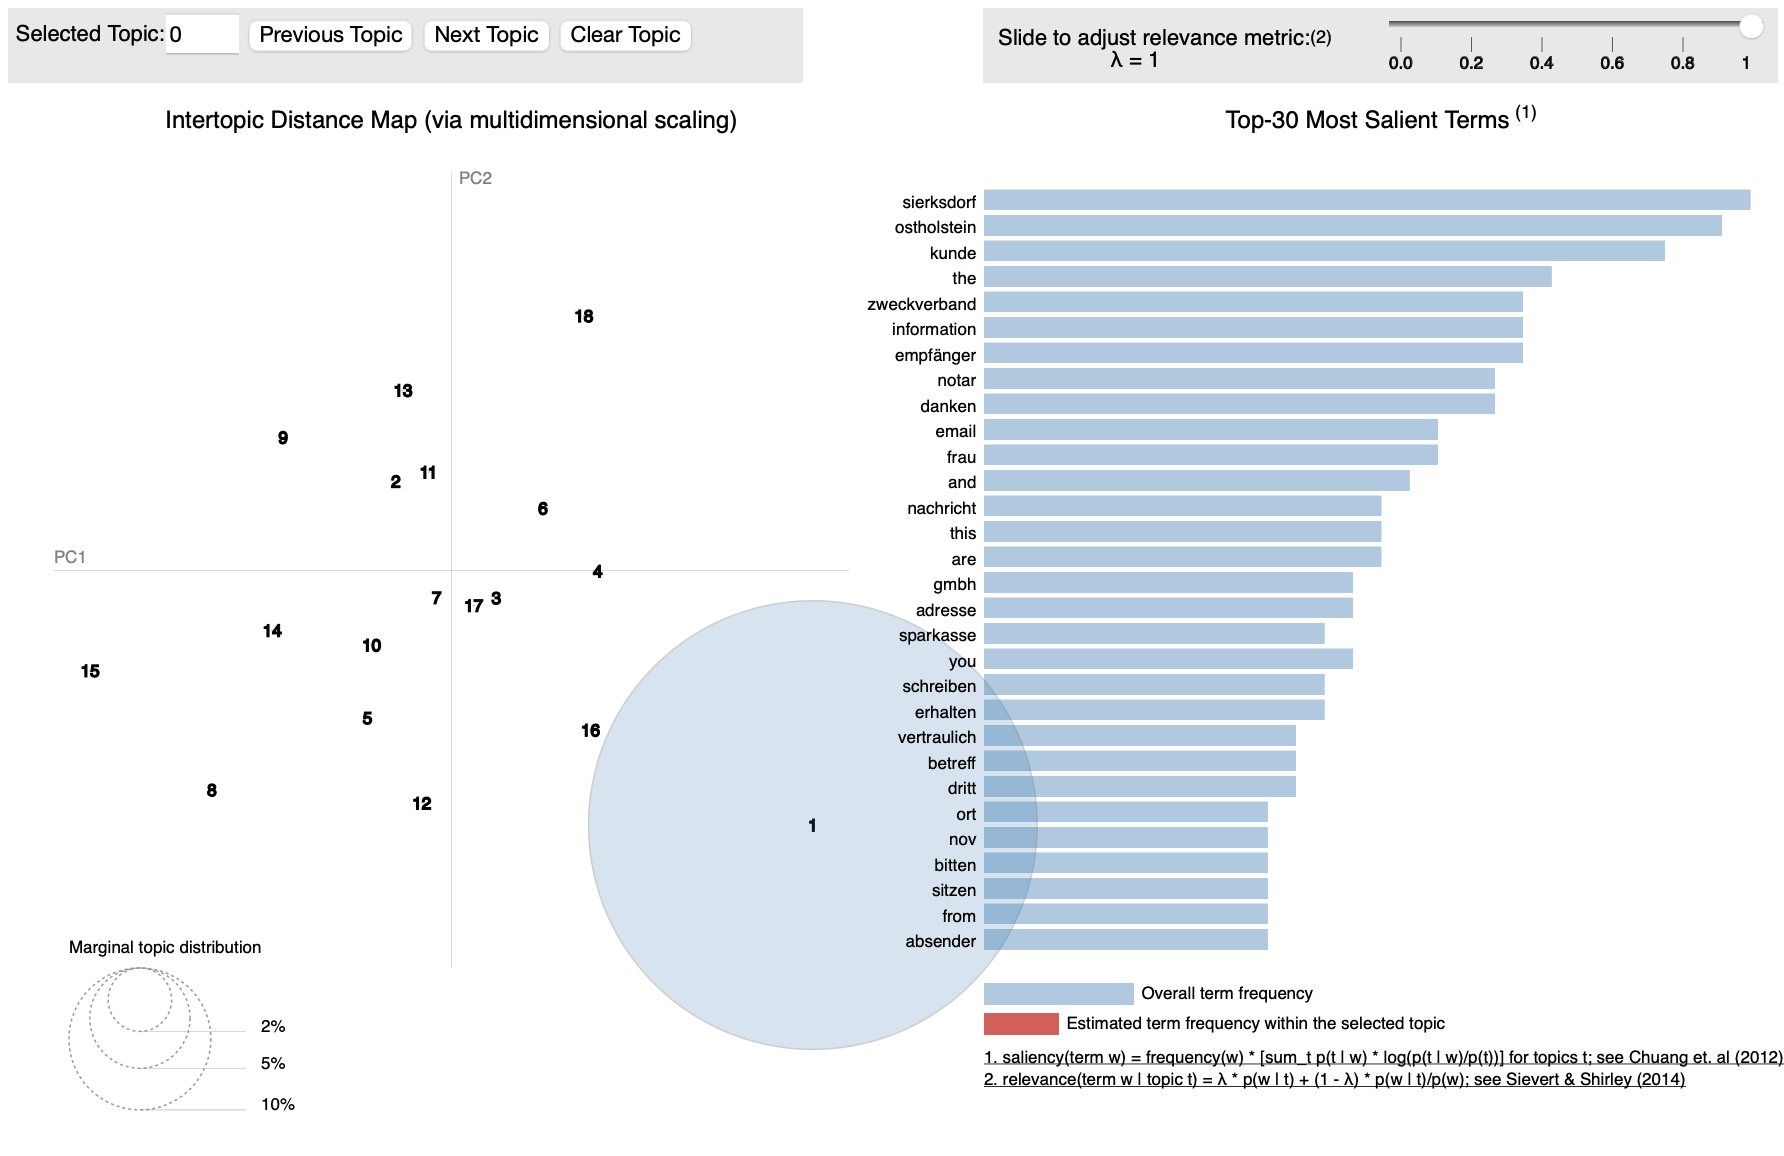
\includegraphics[scale=0.3]{lda_alpha001.png}\\
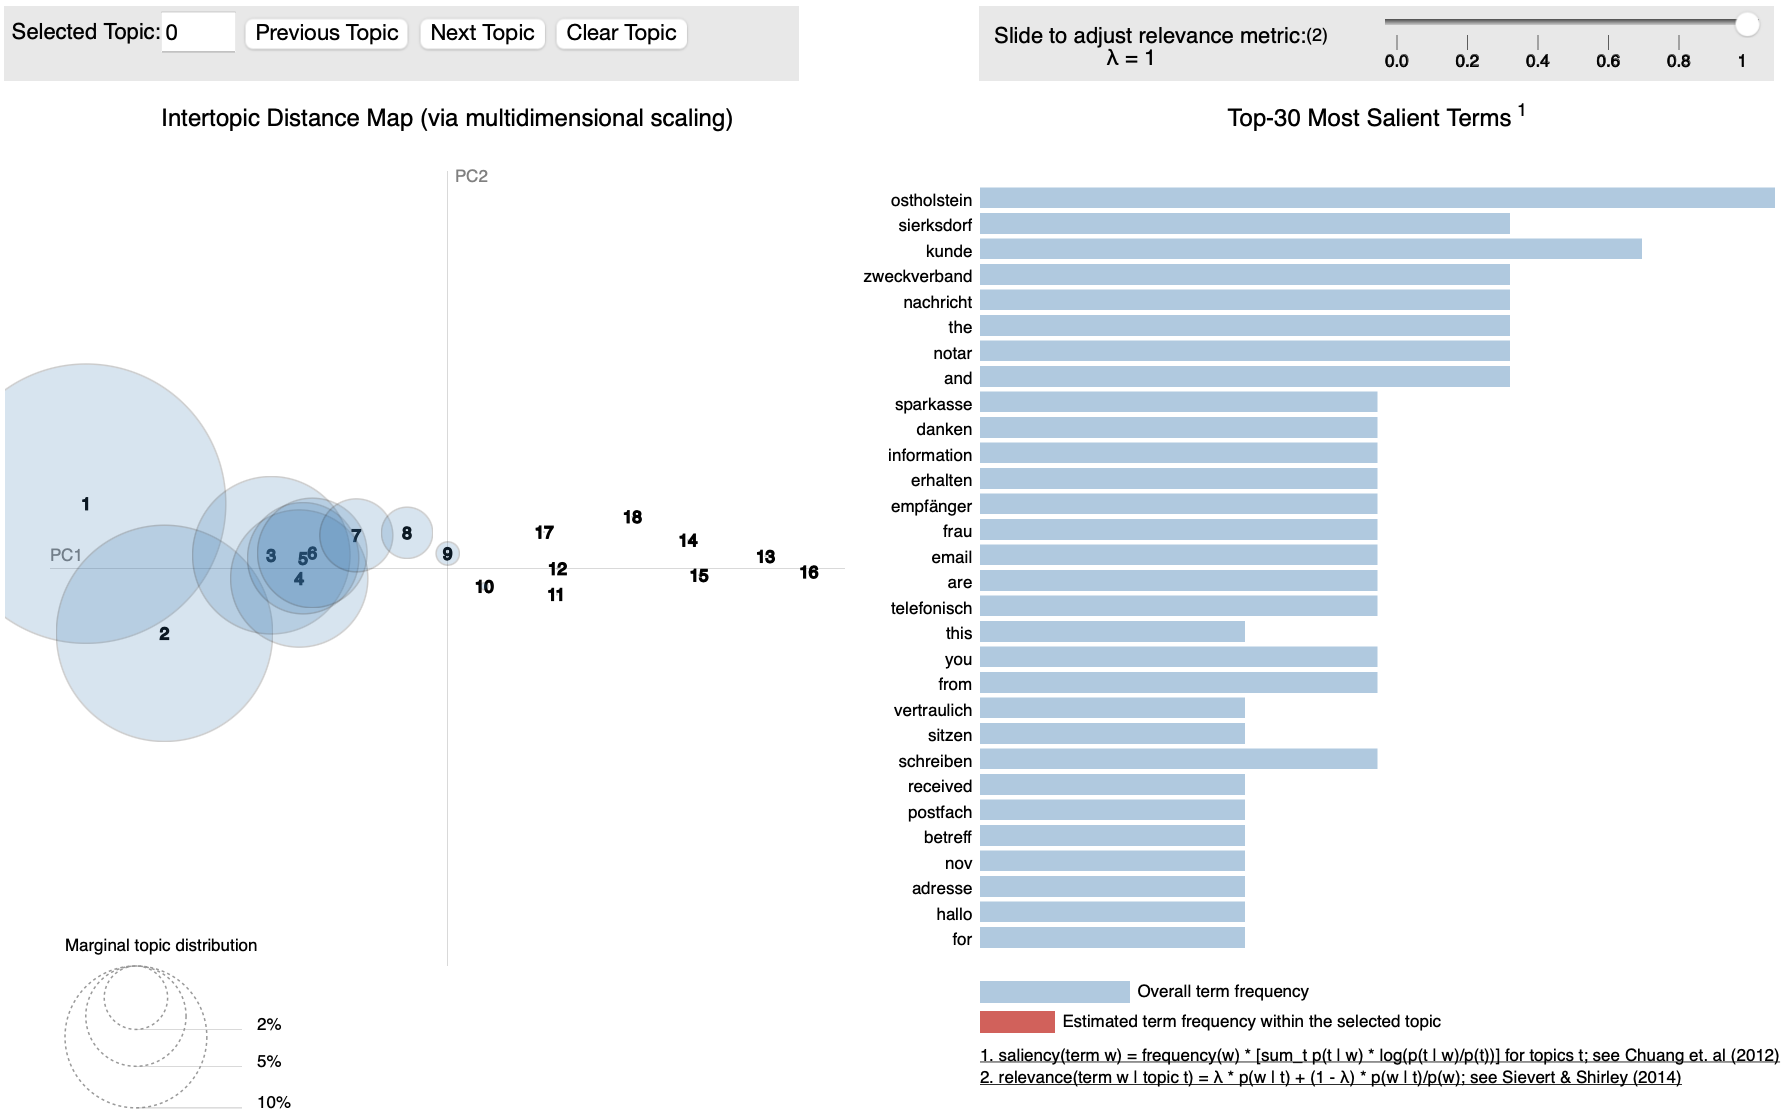
\includegraphics[scale=0.3]{lda_alpha1.png}\\
\end{center}
In der ersten Abbildung führt ein kleiner $\alpha = 0.01$ zu einer sehr eindeutigen Themenvertieilung. Bei der unteren Abbildung hingegen haben wir ein $\alpha = 1$, was eine gleichmäßigere Verteilung zur Folge hat.

%\begin{center}
%\includegraphics{img1.png}
%\end{center}


\section{Daten}
Die Daten liegen in folgendem Format vor: 

%\begin{center}
%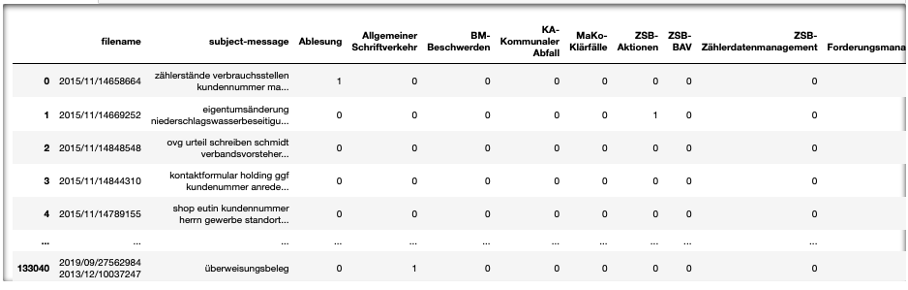
\includegraphics{daten1}
%\end{center}

\begin{center}
\begin{tabular}{ccccccccccc}

\hline
\hline
& filname & subject-message & Abt0 & Abt1 & Abt2 & Abt3 & ... & Abt15 & Abt16 & Abt17\\
\hline
0 & FILE0& content0 &0&0&0&1&...&0&0&0\\
1& FILE1 & content1 &0 &0 &0 &0 &... &1&0&0\\
2& FILE2 & content2 & 1 &0 &0 &0 &...&0 &0&0 \\
3& FILE3 & content3 & 0 & 0  &0 &1 &...&0 &1&0 \\
4& FILE4 & content4 & 0 & 1 &0 &0 &...&0 &0&1 \\
...& ... & ... & ... & ...  &... &... &...&... & ...&... \\
133044& FILE133044 & content133044 & 0 & 0  &1 & 0&...&0 &0&0 \\
\hline
\hline
\end{tabuar}
\end{center}

Relevant für die Auswertung sind die subject-message und die jeweilige Abteilung. Die Tabelle verfügt über eine Matrix mit 18 Abteilungen, von denen pro subject-message eine oder mehrere mit einer 1 versehen ist bzw. sind. Dies beschreibt die Abteilung bzw. Abteilungen, der bzw. denen diese Anfrage manuell zugeordnet wurde. Die Daten in subject-message sind bereits bereinigt, also liegen wie in diesem künstlichen Beispiel vor:\\

%\begin{center}
%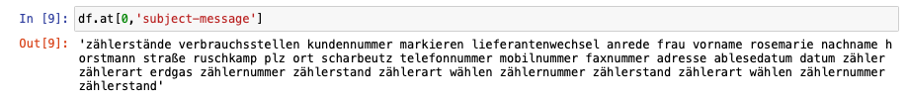
\includegraphics{daten2}
%\end{center}

\begin{lstlisting}
OUTPUT: 
'wasser verbraucht amt deutschland ablesung zaehlen strom voll ort luebeck art straße messung verband nummer platz markieren wechsel lieferant stelle verbrauch kunde kunden anrede mann sommer beschwerde schrift allgemein kommunikation datenmanagement fern'
\end{lstlisting}\\

Um die Einträge in eine computer-lesbare Form zu verwandeln, muss ein Dictionary erstellt werden, dass alle Wörter auf eine Anzahl ihrer Vorkommen abbildet. Dafür müssen die Wörter als alleinige Listeneinträge einlesbar sein: \\

%\begin{center}
%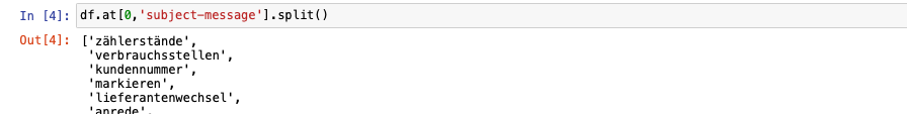
\includegraphics{daten3}
%\end{center}

\begin{lstlisting}
OUTPUT split: 
['wasser', 'verbraucht', 'amt', 'deutschland', 'ablesung', 'zaehlen', 'strom', 'voll', 'ort', 'luebeck', 'art', 'straße', 'messung', 'verband', 'nummer', 'platz', 'markieren', 'wechsel', 'lieferant', 'stelle', 'verbrauch', 'kunde', 'kunden', 'anrede', 'mann', 'sommer', 'beschwerde', 'schrift', 'allgemein', 'kommunikation', 'datenmanagement', 'fern']
\end{lstlisting}\\


\subsection{Datenreinigung}
Bevor eine Themenmodellierung auf Daten durchgeführt werden kann, müssen die Daten einem Prozess unterzogen werden. Dieser beginnt mit der Datenaquise, also der Akquirierung bestimmter relevanter Daten. Im Falle der ZVO bedeutet dies, dass es genügend Kundenanfragen gibt, die verarbeitet werden können. Wenn diese Daten bestehen, werden sie auf die relevanten Wörter reduziert, aus denen eine bedeutsame Inferenz von Informationen möglich ist, sodass unter anderem die sogeneannten „Stop-Words“, also eine Menge von Verbindungswörtern entfernt werden. Ein anderer Schritt der Datenreinigung ist das Transponieren aller Wörter in kleine Buchstaben, um eine Einheitlichkeit zu erlangen, da das Bag of Words Modell keine Reihenfolge mehr beachtet und somit große Satzanfänge irrelevant werden. Wenn die Daten in der gewünschten Form vorliegen, beginnt der Schritt des Featureengineerings. Für einen Computer sind Wörter nicht so leicht zu verarbeiten, wie Zahlen, weshalb in diesem Schritt eine Quantisierung der Wörter und Überführung dieser in eine zahlenbasierte Form vorgenommen wird. Dies kann zum Beispiel in Form eines Bag-of-Words Modells, Dictionary oder TF-IDF, also einer relativen Vorkommensauflistung verschiedner Wörter über Dokumente umgesetzt werden. Nachdem die Daten in eine für den Computer kompatiblen Form gebracht wurden, kann das Themenmodell entwickelt werden. 

\section{Ansätze}
\subsection{Gibbs Sampling}
Gibbs Sampling ist eine Technik, um ein LDA Modell zu trainieren. Für das menschliche Auge kann ein Wort eines Dokuments intuitiv einem Thema zugordnet werden. Für den Computer ist dies schwer, da er die Semantik des Wortes nicht kennt. Mit Gibbs Sampling werden Wörter iterativ Topics zugewiesen basierend auf allen restlichen Wörtern und Dokumenten. Dabei ist zum Einen relevant, was die führende Topic in dem jeweiligen Dokument ist und zum Anderen welcher Topic die gleichen Wörter im gesamten Korpus bereits am häufigsten zugeordnet wurden. Die beiden Beobachtungen werden multipliziert, um die Kombination mit der maximalen Wahrscheinlichkeit zu finden. Um zu verhindern, dass ein Wort einem Topic nicht zugewiesen werden kann, das sich nicht in dem bestimmten Dokument befindet, wird der Anzahl der jeweils vorkommenden Themen im Dokument $\alpha$ und der Anzahl der belegten Themen des gleichen Wörter in anderen Dokumenten $\beta$ addiert.  Wurde ein Wort einem Topic zugewiesen wird das nächste Wort betrachtet. Nun ist zu beachten, dass sich die Verteilungen zur Berechnung jedes mal ändern. Somit haben wir einen iterativen Lernfortschritt bei der Topicverteilung.


\subsection{Hellinger Distanz}
In der Wahrscheinlichkeitsrechnung kann die Hellinger Distanz als Maß genutzt werden, um die Ähnlichkeit zweier Verteilungen zu berechnen. Für diese Anwendung bietet sich die Hellinger Distanz an, da sie oft im Kontext von Modellen und Topics verwendet wird. Zusätzlich lässt sie sich gut in Gensim Implementationen einbauen. Neben der Verteilungsvergleich kann auch eine Hellingermatrix erstellt werden, die jedes Topic des einen Modells mit jedem Topic eines zweiten Modells vergleicht. Somit wird ist es möglich die Ähnlichkeit zwischen zwei Modellen festzustellen. Formal errechnet sich die Distanz zwischen zwei diskreten Verteilungen $X$ und $Y$ aus folgender Gleichung: 

\begin{center}
\begin{equation}
	H(X,Y) = \frac{1}{\sqrt{2}} \sqrt{\sum^k_{i=1}(\sqrt{x_i}-\sqrt{y_i})^2}
\end{equation}
\end{center}

In diesem Abschnitt werden verschiedene Möglichkeiten implementiert und analysiert, wie LDA im Sinne der ZVO genutzt werden kann. Dabei ist die Zielfrage, wie am besten für ein unbekanntes Dokument die bestimmte Abteilung gefunden werden kann. Dafür müssen Korpora bestehen, die bereits durch Verteilung definiert sind, sodass die Dokument-Themen Verteilung für das neues Dokument inferiert werden kann. Wenn die Themenverteilung des neuen Dokuments gegeben ist, kann über Vergleiche der Verteilungen mit Dokumenten oder Durschnitten von Korpora eine Abteilung für das Dokument identifiziert werden. 

Die Möglichkeiten, die sich für diesen Zweck ergeben sind folgende: 
\begin{enumerate}
\item \textbf{Ein großer Korpus}\\
Alle Dokumente ergeben einen Korpus. Dieser gibt eine Dokument-Topic-Verteilung aus, die eine generelle inhaltliche Verteilung der Anfragen darstellt. Neue Dokumente können auf dem Korpus geprüft werden, um eine Dokument-Topic-Verteilung zu inferieren. Diese ergibt eine Abteilung, dem das Dokument zugeordnet werden soll. 

%Ein Gesamtbild der thematischen Aufteilung aller Dokumente kann eine mögliche effektivere Neuverteilung der Kategorien schlussfolgern. Diese Methode stellt die simpleste Form der LDA Anwendung auf die ZVO Daten dar. Dafür kann man zwei verschiedene Ansätze verfolgen: 
%\begin{enumerate}
%	\item Mit 80\% der Daten wird das Modell trainiert. Die letzten 20 \% werden zum Testen verwendet. In diesem Fall wird aus dem unüberwachten LDA-Prinzip ein überwachtes Modell simuliert, da die händisch zugeteilten Abteilungen für die Dokumente bereit bekannt sind. Somit kann man prüfen, wie gut das Modell ist. Dies lässt sich in einer Quote darstellen, die die richtig zugeordneten Dokumente durch die Gesamtanzahl der Testdaten teilt. 
%	\item Mit 80\% der Daten wird das Modell trainiert. In dieser Methode werden jedoch die verwendeten 80\% der Daten verwendet, um zu testen, ob eine Veränderung der Korrektheit zu erkennen ist, wenn die  Trainingsdaten gleichzeitig die Testdaten sind. Dafür wird eine Matrix aufgetellt 
%\end{enumerate}

\item \textbf{18 Korpora mit Durchschnitt}\\
Jede Abteilung stellt einen Korpus da, deren Verteilung mit der des neuen Dokuments verglichen wird. In diesem Fall hat jede der 18 Abteilungen eine Dokument-Themen Verteilung, die die Abteilung inhaltlich von den anderen unterscheidet. Dazu wird ein neues Dokument in jedem einzelnen Korpus integriert, um eine Dokument-Themen Verteilung für das neue Dokument auf Basis der korpusabhängigen Wörter-Themen Verteilung zu inferieren. 

\item \textbf{18 Korpora mit Mehrheitsentscheid}\\
Jede Abteilung stellt einen Korpus dar, deren Dokumente alle einzeln mit der Verteilung des neuen Dokuments verglichen werden, das dann quantitativ einer Abteilung zugeordnet wird. Die Wörter-Themen Verteilung ist für alle dokumente eines Korpus gleich, während für jedes Dokument eine Dokument-Themen Verteilung errechnet wird. Wenn die Dokument-Themen Verteilung der bestehenden Dokumente und die des neuen Dokuments bereitstehen, können diese auf Ähnlichkeit überprüft werden. Da bereits bekannt ist, welcher Abteilung jedes Dokument angehört, stellen die Top X ähnlichsten Dokumente eine Verteilung der Abteilungen dar, denen das neue Dokument inhaltlich am ähnlichsten ist. 
\end{enumerate}



\subsection{Möglichkeit 1: Ein großer Korpus \textcolor{red}{Groppe}}

Alle Dokumente ergeben ein Korpus. Das neue Dokument wird mit dem gesamten Korpus verglichen und auf thematische Kompatibilität geprüft. Dabei sind folgende Prozessschritte notwendig: 

\begin{enumerate}
\item Der Korpus generiert eine Topic-Verteilung für die Gesamtheit aller Dokumente. Dabei werden zuerst alle Anfragedaten in einen String zusammengefügt, der als Grundlage für das Wörterbuch und den Korpus dient. Durch den Aufruf des LDA Modells wird der String in eine vorgegebene Anzahl an Themen eingeteilt, basierend auf häufig zusammen auftretenden Wörtern des Wörterbuchs. Dabei ist an den Topics jedoch keine Verbindung zu den gegebenen Abteilungen ersichtlich. Diese muss zuerst herausgefunden werden, damit die Zuordnung der Dokumente evaluiert werden kann. Die Zuordnung der Topics zu Abteilungen kann nur approximiert werden, indem gezählt wird, in wie vielen Dokumenten sich die Topics und Abteilungen jeweils überschneiden. Für diese Überschneidung wird jedes Dokument erneut auf dem Korpus geprüft, um dessen Topic-Wort-Verteilung zu erstellen. Die Dokumente werden anhand ihrer einzigartigen Zeilen-ID adressiert. Die Überschneidungen werden in einer Matrix dargestellt, die für jede Topic des Modells die Überschneidungen zu jeder Abteilung auflistet. Somit kann für jede Zeile die passende Zuordnung gefunden werden. 

\begin{center}
\begin{tabular}{c c c c c c c c c c c c c c c c c c c}
\hline
& 0 & 1 & 2 & 3 & 4 & 5 & 6 & 7 & 8 & 9 & 10 & 11 & 12 & 13 & 14 & 15 & 16 & 17  \\ 
\hline
0& x & x & x & x & x & x & x & x & x & x & x & x & x & x & x & x & x & x  \\ 
\hline
1 &x & x & x &  x & x & x & x & x & x & x & x & x & x & x & x & x & x & x \\ 
\hline
2& x & x & x & x & x & x & x & x & x & x & x & x & x & x & x & x & x & x  \\ 
\hline
3&x & x & x & x & x & x & x & x & x & x & x & x & x & x & x & x & x & x  \\ 
\hline
4&x  & x & x & x & x & x & x & x & x & x & x & x & x & x & x & x & x & x  \\ 
\hline
5 &x  & x & x & x & x & x & x & x & x & x & x & x & x & x & x & x & x & x  \\ 
\hline
6 &x  & x & x & x & x & x & x & x & x & x & x & x & x & x & x & x & x & x \\ 
\hline
7 & x  &  x & x & x & x & x & x & x & x & x & x & x & x & x & x & x & x & x  \\ 
\hline
8 & x  & x & x & x & x & x & x & x & x & x & x & x & x & x & x & x & x & x  \\ 
\hline
9 & x  & x & x & x & x & x & x & x & x & x & x & x & x & x & x & x & x & x  \\ 
\hline
10 & x  & x & x & x & x & x & x & x & x & x & x & x & x & x & x & x & x & x  \\ 
\hline
11 & x  & x & x & x & x & x & x & x & x & x & x & x & x & x & x & x & x & x  \\ 
\hline
12 & x  & x & x & x & x &x &  x & x & x & x & x & x & x & x & x & x & x & x  \\ 
\hline
13 & x  & x & x & x & x & x &x &  x & x & x & x & x & x & x & x & x & x & x  \\ 
\hline
14 & x  & x & x & x & x & x & x &x &  x & x & x & x & x & x & x & x & x & x  \\ 
\hline
15 & x  & x & x & x & x & x & x & x &x &  x & x & x & x & x & x & x & x & x  \\ 
\hline
16 & x  & x & x & x & x & x & x & x & x &x &  x & x & x & x & x & x & x & x  \\ 
\hline
17 & x  & x & x & x & x & x & x & x & x & x &x &  x & x & x & x & x & x & x \\ 
\hline
\end{tabular}\end{center}\\

Diese Matrix bildet die Überschneidungen der ersten 1000 Dokumenten dar. Die Schwierigkeit besteht darin, ein Mapping zu finden, das in Summe die meisten Überschneidungen ergibt und gleichzeitig jede Abteilung nur genau einem Topic zugeordnet wird. Würde man die zweite Prämisse vernachlässigen, würde sich diese Zuordnung der Topics zu Abteilungen ergeben: 

\begin{lstlisting}[language=Python]
maxmatrix = [9, 10, 0, 9, 10, 10, 0, 10, 10, 0, 1, 2, 1, 9, 10, 9, 10, 9] TODO UPDATEN
\end{lstlisting}

Eine optimale Zuordnung ist erreicht, wenn alle Zahlen von Eins bis 18 ohne Duplikate in der Liste in einer beliebigen Reihenfolge vorkommen. Das würde bedeuten, dass einem Thema von LDA genau eine Abteilung der ZVO am wahrscheinlichsten zugeordnet ist. In der Liste wird jedoch deutlich, dass viele Themen des LDA Modells mit dem 9. und 10. Thema der ZVO kompatibel wären. Bezieht man die Bedingung, eine Abteilung nur einmal zu vergeben, mit ein, ergibt dies folgende Zuordnung, die für die zukünftige Verarbeitung neuer Dokumenten fundamental ist:

\begin{lstlisting}[language=Python]
maxmatrix = []
\end{lstlisting}

\item Ist für jede Abteilung ein Topic-Äquivalent approximiert, kann die Dokument-Topic-Verteilung für ein neues Dokument basierend auf der Topic-Wort-Verteilung errechnet werden. Dafür werden die 20\% der Daten genutzt, die nicht für die Erstellung des Korpus verwendet wurden. Erhält man eine Dokument-Topic-Verteilung für ein neues Dokument, ist aus dieser ersichtlich, welches Topic am stärksten in diesem Dokument vertreten ist. Für das Topic wird die im vorherigen Schritt errechnete Abteilung assoziiert, der das Dokument zugeordnet wird. Um die Korrektheit der Zuordnung prüfen zu können, vergleichen wir die errechnete Abteilung mit der, der die Zeilen-ID des Dokuments in den gegeben Daten zugeordnet ist. Somit wurde eine unüberwachte Lernmethode in eines überwachtes Modell überführt. 

\item Da ein Dokument keine zuverlässige Aussage über die Funktionalität des Modells macht, wird eine Menge an Dokumenten verwendet. Diese ergeben sich aus den letzten 20\%. Um zu prüfen, wie die Anzahl der Testdokumente die Quote der korrekt zugewiesenen Dokumente beeinflusst, wird die Zuordnung mit 5\%, 10\%, 15\% und 20\% durchgeführt. Das Ergebnis ist in der folgenden Abbildung dargestellt:  

\begin{center}
\begin{tabular}{c c}
\hline
Testdaten (in \% von 20\%) & Korrekt zugeordnet \\
\hline
5 & 329/6652 \\
10 & 654/13304 \\
15 & 963/19956\\
20 & 1393/27042 \\ 
\hline
\end{tabular}\\
\\
\\
%HIER NOCHMAL ALS GRAPH 

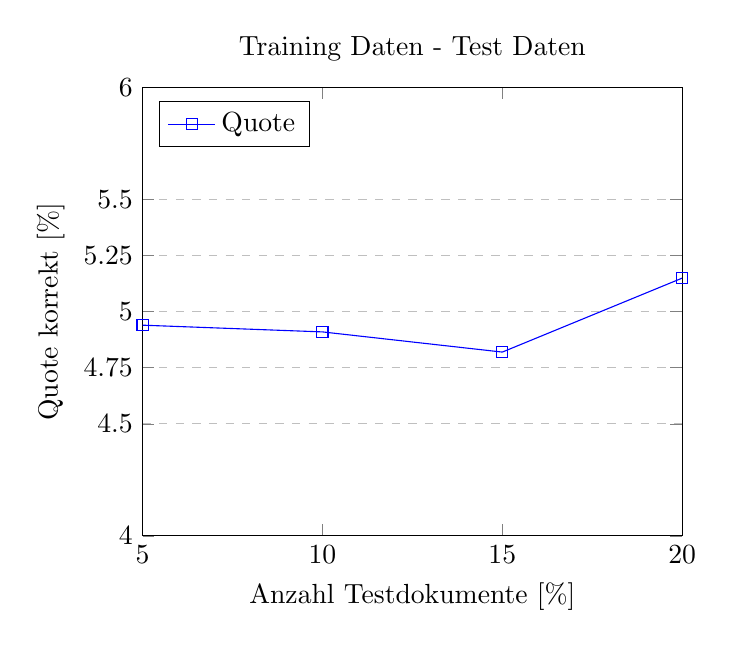
\begin{tikzpicture}
\begin{axis}[
    title={Training Daten - Test Daten},
    xlabel={Anzahl Testdokumente  [\%]},
    ylabel={Quote korrekt [\%]},
    xmin=5, xmax=20,
    ymin=4, ymax=6,
    xtick={5,10,15,20},
    ytick={4,4.5,4.75,5,5.25,5.5,6},
    legend pos=north west,
    ymajorgrids=true,
    grid style=dashed,
]

\addplot[
    color=blue,
    mark=square,
    ]
    coordinates {
    (5,4.94)(10,4.91)(15,4.82)(20,5.15)
    };
    \legend{Quote}
    
\end{axis}
\end{tikzpicture}
\end{center}

\end{enumerate}

Der Versuch zeigt ein sehr schlechtes Ergebnis mit einem Quotendurchschnitt von 4.96. Dabei wurden keine erheblichen Unterschiede bei der Verwendung verschieden vieler Testdaten im Ergebnis festgestellt. Dies lässt zu der Folgerung führen, dass die Nutzung eines einzigen Korpus für die ZVO nicht in Frage kommt. 



\subsection{Möglichkeit 2: 18 Korpora mit Durchschnitt \textcolor{red}{Felix}}
Als weitere Möglichkeit wird aus jeder der 18 vorgegebenen Abteilungen ein eigener Korpus generiert. Somit verfügt jeder Korpus über eine Dokument-Topic-Verteilung, die die Vorkommenswahrscheinlichkeit der 18 Themen in dem jeweiligen Korpus repräsentiert. Ziel der Untersuchung ist die Klassifikationsfähigkeit eines unbekannten Dokuments. Da jeder Korpus aus verschiedenen Dokumenten besteht, gibt es in 18 Korpora auch 18 verschiedene Topic-Word-Verteilungen. Pro Korpus wird für das neue Dokument die Dokument-Topic-Verteilung auf Basis der individuellen Topic-Word-Verteilung generiert. Dafür ist die Dokument-Topic-Verteilung der einzelnen Korpora relevant, die sich aus dem Durchschnitt aller Dokument-Topic-Verteilung der Dokumente eines jeweiligen Korpus ergibt. Aus dem Vergleich der Dokument-Topic-Verteilung des neuen Dokuments mit der des Korpus ergibt sich, wie gut das Dokument zu der Abteilung passt. Dieser Vergleich kann z.B. durch die Berechnung des Hellinger-Abstands der Verteilungen durchgeführt werden. Ist das Ergebnis klein, sind die Verteilungen ähnlich zu einander. Das neue Dokument wird dem Korpus zugeteilt, dessen Abstandsberechnung das minimale Ergebnis zeigt. Um zu analysieren, wie gut das Modell unbekannte Dokumente zuweist, kann nun die berechnetet Abteilung mit dem vorgelabelten Ergebnis verglichen werden. Bei einem Dokument ist das Ergebnis entweder richtig oder falsch, führt man den Vorgang jedoch mit mehreren Dokumenten aus, kann eine Quote errechnet werden. Diese sagt aus, wie gut die Dokumente klassifiziert wurden. 

Das Ergebnis kann sich durch Anpassung der Parameter im Modell verändern. Diese Änderungen werden wir untersuchen. 

\textcolor{red}{Aktuelles Problem: Durschnittsberechnung (hardgecoded) dauert für alle mehrere Tage}\\


\subsection{Möglichkeit 3: 18 Korpora mit Mehrheitsentscheid \textcolor{red}{Felix2}}
Die Unterscheidung dieser Methode zu Möglichkeit 2 ist, dass sich die Topic-Wort-Verteilung eines Korpus nicht aus dem Durchschnitt aller ergibt, sondern das unbekannte Dokument mit allen Verteilungen einzeln verglichen wird. Die Ähnlichkeit wird dann durch die Hellinger-Distanz bestimmt. Dabei berechnet man die Distanz zwischen der Verteilung des neuen Dokuments und der jeden Dokuments enthalten im Korpus. Der Durchschnitt beschreibt die Ähnlichkeit zu dem Korpus und ergibt sich aus der Summe aller Distanzen geteilt durch die Anzahl der Vergleiche. Bei 18 Korpora wird das neue Dokument dem zugeordnet, der die höchste Ähnlichkeit errechnet hat. Als Code wird dies folgendermaßen abgebildet: \\

\begin{lstlisting}

sim = 0

new_doc = df.at[unbekannt_docs_abt0[0], 'subject-message']
bow = corpora.Dictionary([abt0]).doc2bow(new_doc.split())
t_new_doc = lda0.get_document_topics(bow) 

for a in range(18):
    for n in range(len(globals()['index_abt%s' % a])):
        doc = df.at[(globals()['index_abt%s' % a][n]),'subject-message']
        bow = corpora.Dictionary([(globals()['abt%s' % a])]).doc2bow(doc.split())
        t = globals()['lda%s' % a].get_document_topics(bow)
        sim += hellinger(t_new_doc,t)
    sim = sim/len((globals()['index_abt%s' % a]))

\end{lstlisting}\\


Für das in diesem Algorithmus genutztes unbekanntes Dokument wurde diese Ähnlichkeitsliste errechnet: \\

\begin{lstlisting}
sim = [0.18631196155691188, 0.9805342692097637, 0.9596672538794954,  0.9853267249062526, 0.9807896917303207, 0.9872277594688493, 0.9778663668837273,0.9733184898947137, 0.9816813043505935, 0.9712383191132694, 0.9609198366954252, 1.01269095883496, 0.9789156307013527, 0.947041755787613, 0.9751426522996282, 0.9768546403218383, 0.9745868410322677, 0.9810759260918432]
\end{lstlisting}\\


Diese Liste enthält die Stärke der Ähnlichkeit des neuen Dokuments zu den 18 Korpora. Die Hellinger Distanz ist klein, wenn die Argumente ähnlich sind und groß, wenn sie verschieden sind. In der Liste ist der erste Eintrag mit Abstand am geringsten, weshalb das Dokument dem ersten Korpus, also der Abteilung 0 zugeordnet werden würde. Im Algorithmus sieht man, dass das neue Dokument tatsächlich aus Abteilung 0 gewählt wurde. Somit war die Zuordnung erfolgreich. \\

Um eine aussagekräftigere Quote zu erhalten wird dieser Algorithmus für ein unbekanntes Dokument jeden Korpus durchgeführt. Die jeweiligen Zuordnungen werden in einer Liste gespeichert. Der Index besagt aus welchem Korpus ein Dokument entnommen wurde und der Wert, den Korpus, dem es zugeordnet wurde. Das Ergebnis zeigt folgendes: \\

\begin{lstlisting}
assignment= [0,14,2,8,4,5,2,7,3,2, 8,11,12,13,4,15,11,6]
\end{lstlisting}\\
\\
\\

Eine perfekte Zuteilung wäre erreicht, wenn die Liste mit den Zahlen 0 bis 17 in aufsteigender Reihenfolge gefüllt wäre. Die Quote von richtig zugeordneten Dokumenten liegt somit bei 50\%. Bei der korrekten Zuordnung war eine klare Abgrenzung der Distanz gegenüber den inkorrekten Abteilungen festzustellen. Die korrekten Abteilungen hatten eine Distanz von ca $[0.01,0.09]$ . Bei inkorrekten hingegen entschied sich die Zuordnung durch wenige Zehntel Unterschiede in der Ähnlichkeit mit der korrekten Abteilung. 

\subsection{Alternativ zu Möglichkeit 1 (Vermutlich nicht zu verwenden)} Das Ziel ist die Generierung einer Themenverteilung über alle Dokumente im Korpus. Diese könnte Aufschluss über die generelle Kategorien der Abteilungen geben. Dafür müssen zuerst alle Daten in einen großen Korpus vereinigt werden, das ist in der Methode „returnAll()“ implementiert. Danach wird diese in eine Liste aufgeteilt und in ein Dictionary verwandelt. Diese wird dann genutzt um mit der „gensim.models.LdaMulticore()“-Methode in einen LDA Modell verwandelt wird. Für dieses Modell wurde die Themenanzahl auf 18 gesetzt, da dies die aktuelle Anzahl der Themen bei dem ZVO ist. 

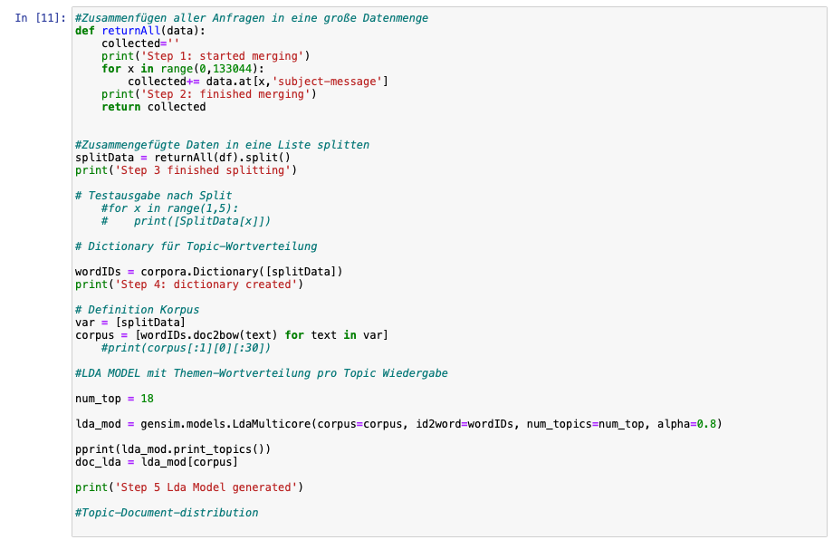
\includegraphics[scale=0.5]{lda1.png}
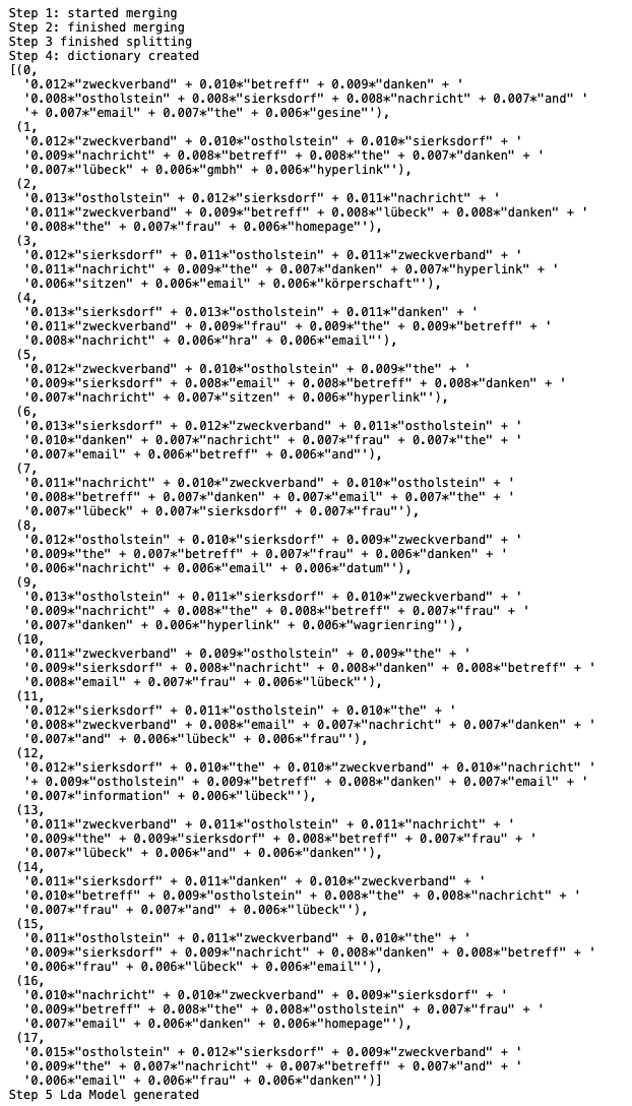
\includegraphics[scale=0.5]{lda2.png}

Der Output zeigt eine Liste mit 18 Elementen. Jedes Element beschreibt die Wortverteilung in einem der 18 Themen. Dabei kann LDA das Thema nicht semantisch benennen, sondern nur Cluster an häufig zusammen vorkommenden Wörtern formen. Daher kommt auch der „Latent“-Teil in der Benennung. Neben der Themen-Wortverteilung ist die Dokument-Themenverteilung von Interessen, also wie häufig kommt jedes Topic in der Gesamtmenge aller Anfragedaten vor. Diese Information errechnet man sich, indem man die folgende Methode aufruft:

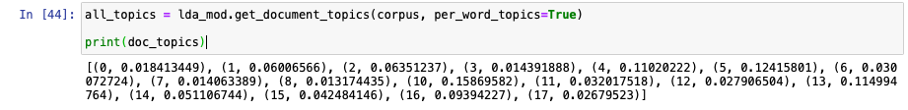
\includegraphics[scale=0.5]{lda3.png}

Aus dieser Ausgabe wird nun ersichtlich, wie wahrscheinlich es ist, dass ein bestimmtes Thema in den Daten vorkommt. Das 10. Thema ist mit 15,9\% das am häufigsten Vorkommende Thema und damit sind die Wörter „zweckverband“, „ostholstein“ und „sierksdorf“ die am stärksten vertretenen Wörter im Gesamtkorpus. Dieses Ergebnis überrascht nur bedingt, da dies der Name der Organisation ist und demensprechend häufig in Anfragen vorkommt. 

Wenn man den gleichen Quelltext mit einer geringeren Themenanzahl aufruft, kommt man auf ein ähnliches Ergebnis, hier mit Beispiel 4: 

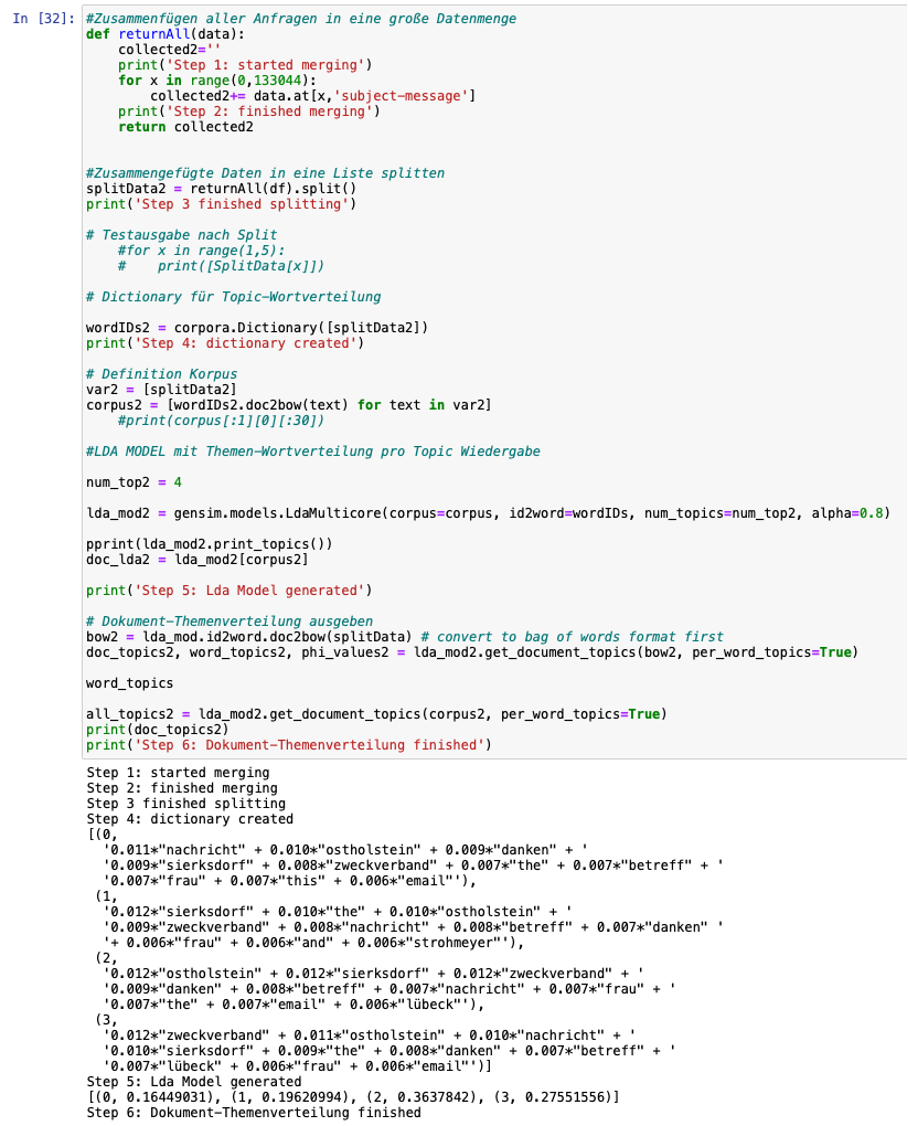
\includegraphics[scale=0.5]{lda4.png}

Wieder hat das meistvertrene Thema die Wörter „zweckverband“, „sierksdorf“ und „ostholstein“ als häufigste vorkommende Elemente. Als Einflussfaktor dient die Dirichlet Variable Alpha, die beeinflusst, wie stark die Wahrscheinlichkeitsunterschiede zwischen den einzelnen Werten ist. Im vorherigen Beispiel war Alpha 0,8 von 1.0. Im folgenden ist es 0,2 von 1.0: 

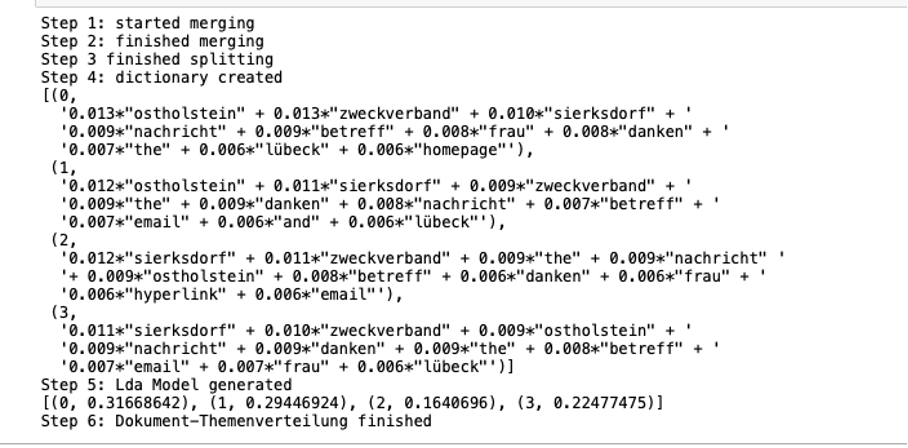
\includegraphics[scale=0.5]{lda5.png}

\textcolor{red}{Was bringt mir das?}

\subsection{\textcolor{red}{Möglichkeit 4 ??}}

\section{Auswertung}
	\subsection{Quellcode}
	\subsection{Perplexität}
	\subsection{ZVO}

	

\chapter{Conclusion}
% In a German thesis write: \subsection{Zusammenfassung und Ausblick}


% !!!!!!!!!!!!!!!!!!!!!!!!!!!!!!!!!!
% !!! Your action is needed here !!!
% !!!!!!!!!!!!!!!!!!!!!!!!!!!!!!!!!!
%
% Replace the following with your conclusion



...



% Normally, the bibliography comes next at this point. Do *not* (try
% to) include further indices and tables like an index or
% a list of figures or a list of tables or such things. Nobody
% actually uses them and they just use up space. 
%
% You *can* however include a glossary, if this seems appropriate. It
% goes here as an unnumbered chapter. Most thesis will *not* need a
% glossary: a well-written text (re)explains strange words and
% concepts as necessary. However, there are situations where a
% glossary may be helpful.














%%%
% 
% Bibliographies
%
%%%
%
% The uzl-thesis class will load biblatex for the bibliography
% management. This is a powerful package, see its documentation for
% details. The styles will be setup correctly and automatically by
% choosing one of the two style keys as described earlier.
%
% In order for the bibliography to work, run latex in the following
% order (which is the standard order):
% 
% > lualatex thesis-example
% > bibtex thesis-example
% > lualatex thesis-example
% 
% Add BibTeX files using \addbibresource or use the {bibtex entries}
% environment (see below).
%
%%%
%
% Although everyting is normally setup automatically, you can change
% the options passed to biblatex using the key 'biblatex';
% for instance,
%
%   \UzLThesisSetup{biblatex={firstinits=false}}
%
% will switch off shortened first names. Normally, you will not need
% this key in your preamble. 
% 
% Note that the bibtex program is used as the 'backend' of biblatex
% by default (rather than biber, which is the preferred program of
% biblatex). This means that you can (and must) run *bibtex* after you
% have run lualatex on your thesis. If you wish to use biber instead
% of bibtex, say 'biblatex={backend=biber}'. 
% 
%%%
%
% The following environment is optional. It allows you to keep the
% bibtex entries for your thesis right here in the thesis file. What
% happens is that each time this tex file is processed, the contents
% of the following environment gets written to the file
% \jobname-bibtex-entries.bib (this file gets overwritten each
% time). Independently, \addbibresource{\jobname-bibtex-entries.bib}
% is always called if the file \jobname-bibtex-entries.bib
% exists. 
%
% In result, you can edit and keep the bibliography's bibtex entries
% right here. If you change something here, run latex, then bibtex,
% then latex once more.
%
% If you would like to manage the bibtex entries in a separate file,
% remove the below environment, delete the \jobname-bibtex-entries.bib
% file and instead write
%
% \addbibresource{filename-of-your-bibtex-file.bib}
%
% in the preamble.
%
%%%


% !!!!!!!!!!!!!!!!!!!!!!!!!!!!!!!!!!
% !!! Your action is needed here !!!
% !!!!!!!!!!!!!!!!!!!!!!!!!!!!!!!!!!
%
% Replace following example entries with the ones of your thesis.

\begin{bibtex-entries}

@Book{Knuth1986,
  author =       {Donald Erwin Knuth},
  title =        {The \TeX book},
  publisher =    {Addison-Wesley},
  year =         {1986},
}

@Book{Lamport1994,
  author =       {Leslie Lamport},
  title =        {\LaTeX: A Document Preparation System},
  publisher =    {Addison-Wesley},
  edition =      {Second edition},
  year =         {1994},
}

@TechReport{Kernighan1974,
  author =       {Brian Kernighan},
  title =        {Programming in C – A Tutorial},
  institution =  {Bell Laboratories},
  year =         {1974}
}

@Manual{Tantau2019,
  author =       {Till Tantau},
  title =        {The Ti\emph kZ and PGF Packages: Manual for version 3.1.3},
  institution =  {Institut für Theoretische Informatik, Universität zu Lübeck},
  year =         {2019},
  url =          {https://github.com/pgf-tikz/pgf}
}

@Book{Alley1996,
  author =       {Michael Alley},
  title =        {The Craft of Scientific Writing},
  publisher =    {Springer},
  year =         {1996},
  edition =      {Third Edition},
}

@Book{DowneyF13,
  author =       {R. G. Downey and M. R. Fellows},
  title =        {Fundamentals of Parameterized Complexity},
  series =       {Texts in Computer Science},
  publisher =    {Springer},
  year =         2013,
  doi =          {10.1007/978-1-4471-5559-1},
}

@Manual{biblatex,
  title =        {The \textsc{BibLaTeX} package},
  subtitle =     {Sophisticated Bibliographies in \LaTeX},
  author =       {Kime, Philip and Lehman, Philipp},
  url =          {https://github.com/plk/biblatex},
  urldate =      {2019-06-11},
  date =         {2018-10-30},
  version =      {3.12}
}

@Manual{varioref,
  title =        {The \textsc{varioref} package},
  subtitle =     {Intelligent page references},
  author =       {Mittelbach, Frank},
  url =          {http://www.ctan.org/pkg/varioref},
  urldate =      {2019-06-11},
  date =         {2016-02-16},
  version =      {1.5c}
}

@Manual{hyperref,
  title =        {The \textsc{hyperref} package},
  subtitle =     {Extensive support for hypertext in \LaTeX},
  author =       {Rahtz, Sebastian and Oberdiek, Heiko},
  url =          {https://github.com/ho-tex/hyperref},
  urldate =      {2019-06-11},
  date =         {2018-11-30},
  version =      {6.88e}
}

@Manual{babel,
  title =        {The \textsc{babel} package},
  subtitle =     {Multilingual support for Plain \TeX\ or \LaTeX},
  author =       {Braams, Johannes L. and Bezos López, Javier},
  url =          {http://www.ctan.org/pkg/babel},
  urldate =      {2019-06-11},
  date =         {2019-06-03},
  version =      {3.32}
}

@Manual{fontspec,
  title =        {The \textsc{fontspec} package},
  subtitle =     {Advanced font selection in Xe\LaTeX\ and Lua\LaTeX},
  author =       {Robertson, Will},
  url =          {http://www.ctan.org/pkg/fontspec},
  urldate =      {2019-06-11},
  version =      {2.7c}
}

@Manual{url,
  title =        {The \textsc{url} package},
  subtitle =     {Verbatim with \textsc{url}-sensitive line breaks},
  author =       {Arseneau, Donald},
  url =          {http://www.ctan.org/pkg/url},
  urldate =      {2019-06-11},
  date =         {2013-09-16},
  version =      {3.4}
}

@Manual{amsmath,
  title =        {The \textsc{amsmath} package},
  subtitle =     {\AmS\ mathematical facilities for \LaTeX},
  author =       {{The \LaTeX\ Team}},
  url =          {http://www.ams.org/tex/amslatex.html},
  urldate =      {2019-06-11}, 
  date =         {2017-09-02},
  version =      {2.17a}
}

@Book{Beutelspacher2009,
  title =        {„Das ist o.\,B.\,d.\,A.\ trivial!“: Tipps und Tricks zur
                  Formulierung mathematischer Gedanken (Mathematik für
                  Studienanfänger)},
  author =       {Albrecht Beutelspacher},
  year =         {2009},
  edition =      {Ninth, updated edition},
  publisher =    {Vieweg+Teubner Verlag},
  doi =          {10.1007/978-3-8348-9075-7},
}

\end{bibtex-entries}



% If you need to have an appendix (I advise against it), insert it
% here using, first, \appendix and then \chapter and then,
% possibly, \section. 
%
% \appendix
%
% \chapter{Technical Appendix}
%
% \section{Experimental Parameters} % possibly
%
% Again, I advise against using an appendix.


\end{document}

%  LocalWords:  LaTeX tex moretexcs Lübeck pdf uzl lualatex bibtex th
%  LocalWords:  TechReport Kernighan Lamport's Tantau's Tantau cls kZ
%  LocalWords:  Mustermann emacs oldschool pdflatex texmf utf biber
%  LocalWords:  biblatex Alphabetische Bibliographie Numerische VIIa
%  LocalWords:  varioref german Einleitung Beiträge dieser Arbeit xml
%  LocalWords:  Ergebnisse Verwandte Arbeiten Aufbau nucleotide VIIc
%  LocalWords:  ensembl amino phylogenetic Alexa Siri decrypt versa
%  LocalWords:  cryptographic pre nondeterministic deterministically
%  LocalWords:  Beutelspacher Untersuchungen zum genetischen sep llcc
%  LocalWords:  Beispiel tikz jpg png Alegrya Kasimir Malewitsch PGF
%  LocalWords:  Lamport Institut für Theoretische Informatik zu url
%  LocalWords:  Universität Springer DowneyF Downey Parameterized doi
%  LocalWords:  BibLaTeX Kime Philipp urldate Mittelbach hyperref Lua
%  LocalWords:  Rahtz Oberdiek Heiko Braams Bezos López fontspec Das
%  LocalWords:  Arseneau amsmath ist Tipps und zur Formulierung
%  LocalWords:  mathematischer Gedanken Mathematik Studienanfänger
%  LocalWords:  Albrecht Vieweg Teubner Verlag
%----------- Unbekanntes Dokument aus Abteilung 2
\begin{comment}
Ähnlichkeit Dokument aus Abteilung 2 new_doc mit Abteilung 0
0.9862926810138586
Ähnlichkeit Dokument aus Abteilung 2 new_doc mit Abteilung 1
0.9571869236469115
Ähnlichkeit Dokument aus Abteilung 2 new_doc mit Abteilung 2
0.4243761541963673
Ähnlichkeit Dokument aus Abteilung 2 new_doc mit Abteilung 3
0.8170893195471294
Ähnlichkeit Dokument aus Abteilung 2 new_doc mit Abteilung 4
0.9874729799815282
Ähnlichkeit Dokument aus Abteilung 2 new_doc mit Abteilung 5
0.9931561753584889
Ähnlichkeit Dokument aus Abteilung 2 new_doc mit Abteilung 6
0.5336300510210132
Ähnlichkeit Dokument aus Abteilung 2 new_doc mit Abteilung 7
0.9835423840076553
Ähnlichkeit Dokument aus Abteilung 2 new_doc mit Abteilung 8
0.9055489259816708
Ähnlichkeit Dokument aus Abteilung 2 new_doc mit Abteilung 9
0.918315655409751
Ähnlichkeit Dokument aus Abteilung 2 new_doc mit Abteilung 10
0.9717280957764937
Ähnlichkeit Dokument aus Abteilung 2 new_doc mit Abteilung 11
1.0200485943384316
Ähnlichkeit Dokument aus Abteilung 2 new_doc mit Abteilung 12
0.9799722682938453
Ähnlichkeit Dokument aus Abteilung 2 new_doc mit Abteilung 13
0.9902009138740018
Ähnlichkeit Dokument aus Abteilung 2 new_doc mit Abteilung 14
0.9448712978582676
Ähnlichkeit Dokument aus Abteilung 2 new_doc mit Abteilung 15
0.853285453931238
Ähnlichkeit Dokument aus Abteilung 2 new_doc mit Abteilung 16
0.9800777378752288
Ähnlichkeit Dokument aus Abteilung 2 new_doc mit Abteilung 17
0.9868668309925873
----------- Unbekanntes Dokument aus Abteilung 3
Ähnlichkeit Dokument aus Abteilung 3 new_doc mit Abteilung 0
0.9546402250634405
Ähnlichkeit Dokument aus Abteilung 3 new_doc mit Abteilung 1
0.9501046677430375
Ähnlichkeit Dokument aus Abteilung 3 new_doc mit Abteilung 2
0.9475955507807069
Ähnlichkeit Dokument aus Abteilung 3 new_doc mit Abteilung 3
0.8203275509481707
Ähnlichkeit Dokument aus Abteilung 3 new_doc mit Abteilung 4
0.9564101798708572
Ähnlichkeit Dokument aus Abteilung 3 new_doc mit Abteilung 5
0.962763088940358
Ähnlichkeit Dokument aus Abteilung 3 new_doc mit Abteilung 6
0.9586901745657708
Ähnlichkeit Dokument aus Abteilung 3 new_doc mit Abteilung 7
0.9530716371514371
Ähnlichkeit Dokument aus Abteilung 3 new_doc mit Abteilung 8
0.81912659051298
Ähnlichkeit Dokument aus Abteilung 3 new_doc mit Abteilung 9
0.9485436573609711
Ähnlichkeit Dokument aus Abteilung 3 new_doc mit Abteilung 10
0.9489000910471992
Ähnlichkeit Dokument aus Abteilung 3 new_doc mit Abteilung 11
0.9880846832670455
Ähnlichkeit Dokument aus Abteilung 3 new_doc mit Abteilung 12
0.9542904546015017
Ähnlichkeit Dokument aus Abteilung 3 new_doc mit Abteilung 13
0.958165395915207
Ähnlichkeit Dokument aus Abteilung 3 new_doc mit Abteilung 14
0.946601483319905
Ähnlichkeit Dokument aus Abteilung 3 new_doc mit Abteilung 15
0.9290476335509387
Ähnlichkeit Dokument aus Abteilung 3 new_doc mit Abteilung 16
0.9488928818477043
Ähnlichkeit Dokument aus Abteilung 3 new_doc mit Abteilung 17
0.9552382581661794
----------- Unbekanntes Dokument aus Abteilung 4
Ähnlichkeit Dokument aus Abteilung 4 new_doc mit Abteilung 0
0.9839514363285209
Ähnlichkeit Dokument aus Abteilung 4 new_doc mit Abteilung 1
0.8354915628775844
Ähnlichkeit Dokument aus Abteilung 4 new_doc mit Abteilung 2
0.972318475461502
Ähnlichkeit Dokument aus Abteilung 4 new_doc mit Abteilung 3
0.9915257842072557
Ähnlichkeit Dokument aus Abteilung 4 new_doc mit Abteilung 4
0.03325975046028289
Ähnlichkeit Dokument aus Abteilung 4 new_doc mit Abteilung 5
0.9841236015589845
Ähnlichkeit Dokument aus Abteilung 4 new_doc mit Abteilung 6
0.6232323879458616
Ähnlichkeit Dokument aus Abteilung 4 new_doc mit Abteilung 7
0.9836855987617704
Ähnlichkeit Dokument aus Abteilung 4 new_doc mit Abteilung 8
0.9879726956648679
Ähnlichkeit Dokument aus Abteilung 4 new_doc mit Abteilung 9
0.9202843331970301
Ähnlichkeit Dokument aus Abteilung 4 new_doc mit Abteilung 10
0.9373869579957838
Ähnlichkeit Dokument aus Abteilung 4 new_doc mit Abteilung 11
1.018147207280227
Ähnlichkeit Dokument aus Abteilung 4 new_doc mit Abteilung 12
0.8841344473377906
Ähnlichkeit Dokument aus Abteilung 4 new_doc mit Abteilung 13
0.9151038193984281
Ähnlichkeit Dokument aus Abteilung 4 new_doc mit Abteilung 14
0.9813243338224691
Ähnlichkeit Dokument aus Abteilung 4 new_doc mit Abteilung 15
0.9739033570519001
Ähnlichkeit Dokument aus Abteilung 4 new_doc mit Abteilung 16
0.9650038868307649
Ähnlichkeit Dokument aus Abteilung 4 new_doc mit Abteilung 17
0.6152921391535795
----------- Unbekanntes Dokument aus Abteilung 5
Ähnlichkeit Dokument aus Abteilung 5 new_doc mit Abteilung 0
0.9683745511670415
Ähnlichkeit Dokument aus Abteilung 5 new_doc mit Abteilung 1
0.9562579997342372
Ähnlichkeit Dokument aus Abteilung 5 new_doc mit Abteilung 2
0.9734004705950261
Ähnlichkeit Dokument aus Abteilung 5 new_doc mit Abteilung 3
0.9891193261219854
Ähnlichkeit Dokument aus Abteilung 5 new_doc mit Abteilung 4
0.9824404824310721
Ähnlichkeit Dokument aus Abteilung 5 new_doc mit Abteilung 5
0.06112917743764569
Ähnlichkeit Dokument aus Abteilung 5 new_doc mit Abteilung 6
0.9865532722447153
Ähnlichkeit Dokument aus Abteilung 5 new_doc mit Abteilung 7
0.9802884380055117
Ähnlichkeit Dokument aus Abteilung 5 new_doc mit Abteilung 8
0.856042711885809
Ähnlichkeit Dokument aus Abteilung 5 new_doc mit Abteilung 9
0.9799059839753889
Ähnlichkeit Dokument aus Abteilung 5 new_doc mit Abteilung 10
0.9730939990637961
Ähnlichkeit Dokument aus Abteilung 5 new_doc mit Abteilung 11
1.0169799125851966
Ähnlichkeit Dokument aus Abteilung 5 new_doc mit Abteilung 12
0.9780887776302069\end{comment}